\subsection{Glissando Effekt}\label{subsec:Glissando_Effekt}
Auch für den Glissando-Effekt war es nötig einen Test durchzuführen um die Genauigkeit der Töne festzustellen. Wir verwendeten dazu anstatt unseres PCB einen Funktionsgenerator, da keine genaue Messung mit dem PCB möglich ist. Um die Frequenz einzustellen, wurde das Tool \textit{SignalTap Logic Analyzer} in Quartus eingesetzt um auf das Register der Frequenzmessung mit den Messresultaten zugegriffen. Schlussendlich wurde der Ton mit der App \textit{Tonal Energy Tuner} auf dessen Genauigkeit gemessen. Die App gibt diese Genauigkeit direkt in Cent an. Die Messung umfasst alle Frequenzen aus der Tabelle \ref{tab:Toene_Frequenzen} in Kapitel \ref{subsec:Musiktheorie}. In Abbildung \ref{img:Validierung_Glissando} sind alle diese Abweichungen aufgezeigt. Die blaue Kurve  zeigt die Resultate, wenn die Frequenz kleiner eingestellt wurde als der anzunähernde Ton. Die orange Kurve zeigt die Resultate, wenn die Frequenz grösser eingestellt wurde als der anzunähernde Ton. Wie zu sehen ist, ist auch diese Funktion genauer als \SI{10}{Cent}.


\begin{figure}[h!]
	\centering
	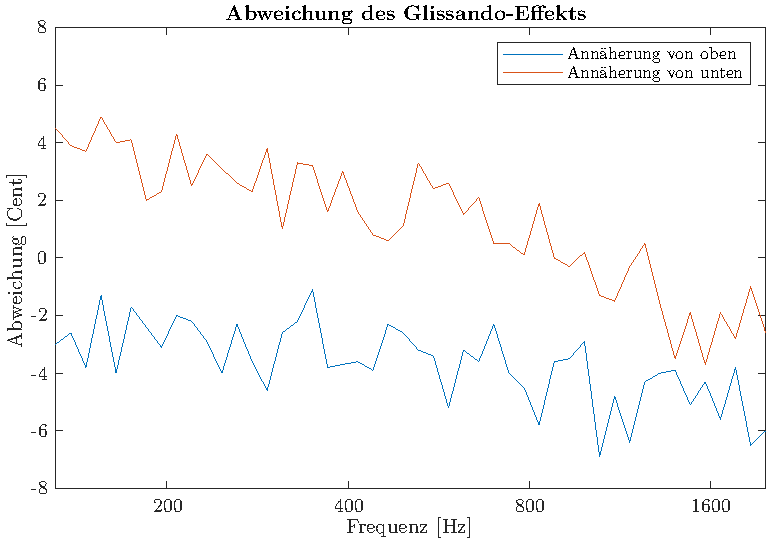
\includegraphics[width=0.9\textwidth]{Validierung_Glissando.pdf}
	\caption{Resultate der Validierung des Glissando-Effekts} 
	\label{img:Validierung_Glissando}
\end{figure}  

\begin{table}[H]
	\centering
	\caption{Clockfrequenzen der verschiedenen Komponenten}
	\label{tab:clocks}
	\begin{tabular}{l|l|l}
		\textbf{Messmittel} & \textbf{Bezeichnung} \\
		\hline\hline
		Funktionsgenerator & MSZ-M-0051   \\ \hline
		SignalTap Logic Analyzer & -    \\ \hline
		Tonal Energy Tuner App &  -   \\ \hline
		
	\end{tabular}
\end{table}

